\subsection{Hyperledger Composer}
        Hyperledger Composer ist ein Framework für das bauen, operieren und deployen von Blockchain-Netzwerken (genannt Business Networks) und dient vornehmlich als Abstraktion des Hyperledger Fabric Frameworks. 
        
        Für die Entwicklung der Logik von Business Networks wird die Sprache JavaScript verwendet. 
        Zusätzlich werden domainspezifische Sprachen für die Modellierung, sowie Access Control eingesetzt.
        Als Datenbank wird CouchCB verwendet (eventual Consistency, bei CAP auf A und P ausgelegt.)
        
        Kleine Beispielapplikation mit generierter Angular-App(?)
        
        \begin{itemize}[noitemsep]
            \item Ein Blockchain-Netzwerk wird Business Network genannt. 
            \item Die Business Network Definition definiert das Datenmodell, die Transaktionslogic und die Regeln für die Zugriffskontrolle.
            \item Ein Business Network besteht aus Assets, Participants, Transactions, Access Control Tules und optional Events und/\-oder Queries.
                Metadaten wie Dependencies und Versionsnummern werden in einer separaten Datei (\colorbox{light-gray}{\lstinline|package.json|}) abgelegt.
        \end{itemize}
        
        \begin{itemize}[noitemsep]
            \item Bietet die Möglichkeit eine REST-\gls{api} pro Business Network Card zu nutzen
                \begin{itemize}[noitemsep]
                    \item Nutzen eines API-Keys für die Sicherung der REST-\gls{api}
                    \item Authentifizierung via Passport (Linux)
                    \item Explorer Test Interface, welches automatisch generiert wird und essentiell eine Dokumentation der \gls{api} darstellt
                    \item Key für dynamisches Logging
                    \item Event publication via WebSocket
                    \item TLS für die \gls{api}
                \end{itemize}
            \item Bietet die Möglichkeit eine simple Anuglar-App zu generieren, welche letztendlich nur eine GUI-Maske für die \gls{api}-Methoden ist.
            \item Actors im Netzwerk (Peers, Orderers, Client Applications etc. haben eine digitale Identität, welche sich in einem X.509 digitalem Zeritifikat befindet.
                Die Zertifikate sind letztendlich ausschlaggebend für die Zugriffskontrolle und den Rechten, die eine Entität in dem Netzwerk erhält. 
                Zusätzlich können weitere Attribute, die zu einer Identät gehören genutzt werden (wie bspw. Organisiation, Rolle, etc.), welche eine Rolle bei der Bestimmung, welche Rechte diese Entität erhalten soll, spielen können.
            \item Zertifikate kommen von einer vertrausenswürdigen Autortität, dem \gls{msp}. 
                Gleicht einer PKI mit digitalen Zertifikaten, public/\-private Keys, CA und CRL
            \item Channels: Nachrichtenwege, um Privatsphäre von Transaktionen und Vertraulichkeit zu gewährleisten.
                Sind nur für bestimmte Netzwerkmitglieder sichtbar, denen der Channel freigegeben wurde.
            \item Ordering Service: Menge an Knoten, die Transaktionen in einem Block ordnen
            \item Ledger: Blockchain + World State
            \item Deployable: Business Network Archive (bna)
            \item Historian: registry which records successful transactions, including the participants and identities that submitted them
        \end{itemize}
        
        \begin{itemize}[noitemsep]
            \item Single Organization 
            \item Membership Provider Service
        \end{itemize}
    
\subsection{Architektur und Funktionsweise}
\label{sec:prototype_arch}
    Enstprechend dem Kapitel mit dem Stand der Wissenschaft wurden die Konzepte im Framework umgesetzt.
    Ausgehend von der Dokumentation des Frameworks \cite{ComposerDocs} wurde die Architektur ausgearbeitet. 
    
    Keine Standardisierung und Best Practices von Architekturen, wie in fast allen Bereichen des \gls{iot}, daher eigentlich völlig frei.
    
    CouchDB ist CAP auf CP ausgelegt.
    
    \begin{figure}[H]
		\centering
		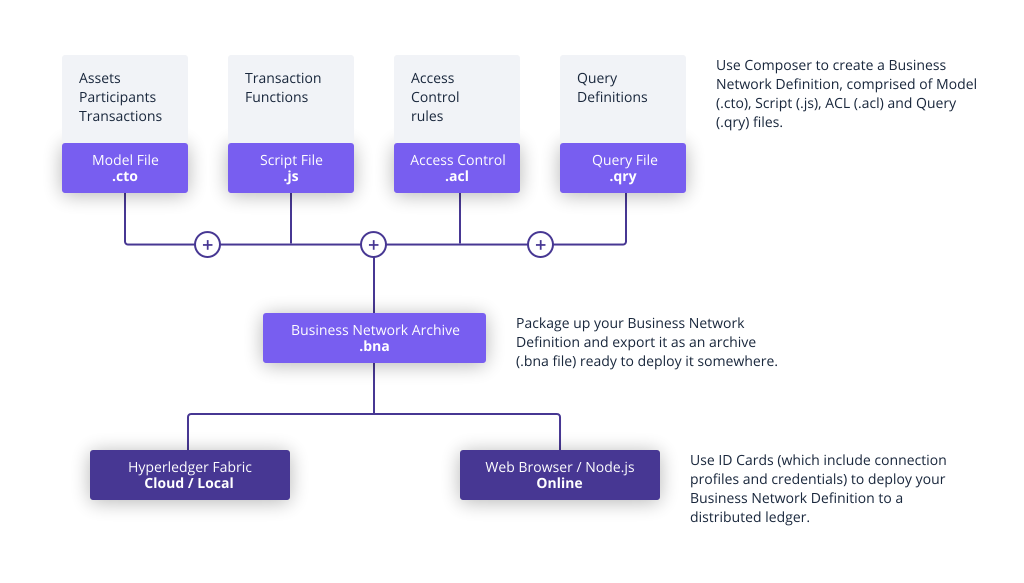
\includegraphics[width=\textwidth]{graphics/Composer-Diagram.png}
		\caption[Bestandteile einer Hyperledger Composer-Applikation]{Bestandteile einer Hyperledger Composer-Applikation\cite{ComposerDocs}}
		\label{fig:composer_arch}
	\end{figure}
    
    Notizen für den Prototypen:
    \begin{itemize}[noitemsep]
        \item Ein Asset als Token für (,,du darfst die Tür aufmachen``) je berechtigtem Nutzer \textrightarrow\ zurückverfolgbar (Accountability)
        \item Framework bietet in irgendeiner Form Access Control an?
        \item How to ensure a consistent state across all entities?...
        \item Vendor Server als Teilnehmer im Netzwerk oder nicht?
        \item Vertraulichkeit überhaupt irgendwie möglich oder durch das Konzept der Blockchain schon gar nicht?
        \item Pseudo-/Anonymisierung der Teilnehmer sinnvoll?
        \item Hyperledger biete CA für Identitäten, Authentifizierung
        \item \begin{itemize}
            \item erlaubt Sicherheitseinstellungen beim Erstellen des REST-API-Servers
            \item API Key
            \item Authentication mit Passport
            \item explorer Test interface ?
            \item dynamic logging
            \item event publication over websockets
            \item TLS enable/\-disable
        \end{itemize}
    \end{itemize}
    
    \subsubsection{Konzept}
    
    \paragraph{Model File}
        Asset Types:
        \begin{itemize}[noitemsep]
            \item Door Key (kann zeitlich beschränkt sein), bei Öffnen an Schloss senden, bei Schließen wieder an Nutzer zurück \textrightarrow\ man kann sich sicher sein, dass die Tür bei 0 Token geschlossen ist.
            \item Token, der die Rolle repräsentiert?
            \item Um \gls{dos} zu vermeiden, etwas ähnliches wie Mutex-Token? z.B. wenn Tür offen ist, dann hat sie genau diesen einen Token
            \item Assets können auch zu anderen Assets oder Teilnehmern eine Beziehung haben\cite{ComposerDocs}
        \end{itemize}
        
        Participant Types:
        \begin{itemize}[noitemsep]
            \item Manufacturer
            \item Owner
            \item Guest
        \end{itemize}
        \begin{lstlisting}[caption={Participant Types (TODO)},label=participants,captionpos=b]
asset Commodity identified by tradingSymbol {
    o String tradingSymbol
    o String description
    o String mainExchange
    o Double quantity
    --> Trader owner
}
participant Trader identified by tradeId {
    o String tradeId
    o String firstName
    o String lastName
}
transaction Trade {
    --> Commodity commodity
    --> Trader newOwner
}
        \end{lstlisting}
        
        
        Transaction Types (entpricht den Funktionen, die man je nach Rolle ausführen darf):
        \begin{itemize}[noitemsep]
            \item OpenDoor
            \item User (AddUser, DeleteUser, ChangeUserRole)
            \item TimeSlot (AddTimeSlot, DeleteTimeSlot, ChangeGuestTimeSlot)
        \end{itemize}
    
    \paragraph{Transaction Functions}
    
    \paragraph{Access Control Rules}
        \begin{itemize}
            \item Whitelisting
        \end{itemize}
    
    \paragraph{Query Definitions}
    
    Rollenbasiertes Zugriffskonzept
    \begin{itemize}[noitemsep]
        \item 
    \end{itemize}